\documentclass[12pt]{article}
\usepackage{amsfonts}

%%%%%%%%%%%%%%%%%%%%%%%%%%%%%%%%%%%%%%%%%%%%%%%%%%%%%%%%%%%%%%%%%%%%%%%%%%%%%%%%%%%%%%%%%%%%%%%%%%%
\usepackage{amsmath,amssymb,amsthm}
\usepackage{multicol}
\usepackage{color}
\usepackage{hyperref}
\usepackage{graphicx}
\usepackage[english]{babel}

%TCIDATA{OutputFilter=Latex.dll}
%TCIDATA{LastRevised=Mon Oct 10 18:16:16 2011}
%TCIDATA{<META NAME="GraphicsSave" CONTENT="32">}
%TCIDATA{CSTFile=article.cst}

\newtheorem{Def}{Definition}[section]
\newtheorem{theorem}{Theorem}
\newtheorem{statement}{Statement}
\newtheorem{Cnj}[Def]{Conjecture}
\newtheorem{Prop}[Def]{Property}
\newtheorem{example}{Example}[section]

\newcommand{\co}[1]{\stackrel{\circ }{#1}}
\newcommand{\gf}{\mathfrak{g}}
\newcommand{\nfp}{\mathfrak{n}^{+}}
\newcommand{\nfm}{\mathfrak{n}^{-}}
\newcommand{\af}{\mathfrak{a}}
\newcommand{\uf}{\mathfrak{u}}
\newcommand{\sfr}{\mathfrak{s}}
\newcommand{\aft}{\widetilde{\mathfrak{a}}}
\newcommand{\afb}{\mathfrak{a}_{\bot}}
\newcommand{\hf}{\mathfrak{h}}
\newcommand{\hfb}{\mathfrak{h}_{\bot}}
\newcommand{\pf}{\mathfrak{p}}

\newcommand{\gfh}{\hat{\mathfrak{g}}}
\newcommand{\afh}{\hat{\mathfrak{a}}}
\newcommand{\sfh}{\hat{\mathfrak{s}}}
\newcommand{\bff}{\mathfrak{b}}
\newcommand{\hfg}{\hf_{\gf}}

%\input{tcilatex}

\begin{document}
\title{On affine extension of splint root systems}



\author{V.D.~Lyakhovsky$^1$, A.A.~Nazarov$^{1,2}$ \\
  {\small $^1$ Department of High-energy and elementary particle physics, SPb State University}\\
  {\small 198904, Saint-Petersburg, Russia}\\
  {\small e-mail: lyakh1507@nm.ru}\\
  {\small$^{2}$ Chebyshev Laboratory,}\\
  {\small Department of Mathematics and Mechanics, SPb State University}\\
  {\small 199178, Saint-Petersburg, Russia}\\
  {\small email: antonnaz@gmail.com}}
\maketitle

\begin{abstract}
Splint of root system of simple Lie algebra appears naturally in
the study of (regular) embeddings of reductive subalgebras. It can
be used to derive branching rules. Application of
splint properties drastically simplifies calculations of
branching coefficients. We study affine extension of splint root system of simple Lie algebra.
\end{abstract}

\section{Introduction}
\label{sec:introduction}


The term {\it splint} was
introduced by D. Richter in  \cite{richter2008splints} where the
classification of splints for simple Lie algebras was obtained.
There was also mentioned that splint must have tight
connections with the injection fan construction. The fan $\Gamma
\subset \Delta$ was
introduced in \cite{lyakhovsky1996rra} as a subset of root system describing recurrent
properties of branching coefficients for maximal embeddings. Injection fan is an
efficient tool to study branching rules. Later this construction
was generalized to non-maximal embeddings and affine Lie algebras
Lie algebras in \cite{2010arXiv1007.0318L, ilyin812pbc}.

In paper \cite{2011arXiv1111.6787L} we have shown that existence of splint of root system of simple Lie algebra leads to simplification of reduction of Lie algebra module to modules of subalgebra. This statement is based upon the properties of injection fan and singular element of Lie algebra module. 

In present note we discuss the poss applications of splint of root system of simple Lie algebra to representation theory of affine Lie algebras. We discuss the structure of injection fan for affine Lie algebras and show that it admits decomposition similar to that used in \cite{2011arXiv1111.6787L} for simple Lie algebras. But there is no such decomposition for singular elements due to semidirect product structure of Weyl group of affine Lie algebras. So there is no straightforward generalization of the coincidence of branching coefficients to weight multiplicities, and branching functions for affine Lie algebras in general do not coincide with string functions of other algebras. 

Then we study graded branching of affine Lie algebra module to finite-dimensional subalgebras and discuss the consequences of splint existence on branching functions in this case. 

\section{Definitions}
\label{sec:definitions}

Consider simple Lie algebra $\gf$ with root system $\Delta$. Let $\af_{1}\subset \gf$ be its reductive subalgebra, such that $\Delta_{1}\subset\Delta$. Irreducible highest-weight modules of $\gf$ and $\af$ are denoted by $L^{\mu}$ and $L^{\nu}_{\af}$ correspondingly. Weyl character formula for irreducible modules is $\mathrm{ch}L^{\mu}=\frac{\Psi^{(\mu)}}{\prod_{\alpha\in\Delta}(1-e^{-\alpha})}$, where $\Psi^{(\mu)}=\sum_{w\in W}\epsilon(w) e^{w(\mu+\rho)-\rho}$ is singular element of the module and $W$ -- Weyl group of $\gf$. Formal character of irreducible module admits decomposition
\begin{equation}
  \label{eq:4}
  \mathrm{ch} L^{\mu}=\sum_{\nu\in P_{\af}} b^{\mu}_{\nu} \mathrm{ch} L^{\nu}_{\af},
\end{equation}
where $P$, $P_{\af}$ are weight lattices of $\gf$ and $\af$.
We want to study affine extension of this situation: $\gf\subset\gfh,\; \af\subset\afh$, $\afh\subset\gfh$, $\hat{\Delta}\subset\hat{\Delta}$ and $\mathrm{ch}L^{\hat{\mu}}_{\gfh}=\sum_{\hat{\nu}} b^{\hat{\mu}}_{\hat{\nu}} \mathrm{ch} L^{\hat{\nu}}_{\afh}$. For weights of affine Lie algebra $\gfh$ we have $\hat{\mu}=(\mu,k,n)$, where $\mu$ is a weight of $\gf$, $k$ -- level of module and $n$ -- grade of weight $\hat{\mu}$

\begin{Def}
Embedding $\phi$ of a root system $\Delta_1$ into a root system $\Delta$ is a bijective map of roots of $\Delta_{1}$ to a (proper) 
subset of $\Delta$ that commutes with vector composition law in $\Delta_{1}$ and $\Delta$.
\begin{equation*}
\phi:\Delta_1 \longrightarrow \Delta
\end{equation*}
\begin{equation*}
\phi \circ (\alpha + \beta) =\phi \circ \alpha + \phi \circ \beta,
\,\,\, \alpha,\beta \in \Delta_1
\end{equation*}
  
\end{Def}

Note that the image $Im(\phi)$ must not inherit the root system properties except the addition rules equivalent to the addition
rules in $\Delta_{1}$ (for pre-images). Two embeddings $\phi_1$ and $\phi_2$  can splinter $\Delta$  when the latter can be presented as a disjoint union of images $Im(\phi_1)$ and $Im(\phi_2)$.   

$\phi$ induces an injection of formal algebras $:{\mathcal{E}}_0
\hookrightarrow \mathcal{E}$ and for the image ${\mathcal{E}}%
_i=Im_{\phi}\left( {\mathcal{E}}_0\right)$ one can consider its inverse $%
\phi^{-1}:{\mathcal{E}}_i \longrightarrow {\mathcal{E}}_0$.

\begin{Def}
A root system $\Delta $ ''splinters'' as $(\Delta _{1},\Delta _{2})$ if there are two embeddings $\phi _{1}:\Delta _{1}\hookrightarrow \Delta $ and $%
\phi _{2}:\Delta _{2}\hookrightarrow \Delta $ where (a) $\Delta $ is the disjoint union of the images of $\phi _{1}$ and $\phi _{2}$ and (b) neither the rank of $\Delta _{1}$ nor the rank of $\Delta _{2}$ exceeds the rank of $%
\Delta $.
\end{Def}

It is equivalent to say that $(\Delta_1,\Delta_2)$ is a "splint'' of $\Delta$ and we shall denote this by $\Delta \approx (\Delta_1,\Delta_2)$. Each component $\Delta_1$ and $\Delta_2$ is a "stem'' of the splint $%
(\Delta_1,\Delta_2)$.

We consider the case when one of the stems $\Delta _{1}=\Delta _{\frak{a}}$ is a root subsystem. As shown in paper \cite{2011arXiv1111.6787L} the second stem $\Delta _{\frak{s}}:=\Delta
_{2}=\Delta \setminus \Delta _{\frak{a}}$ can be translated into a product 
$\prod_{\beta \in \Delta _{\frak{s}}^{+}}\left( 1-e^{-\beta }\right)=-\sum_{\gamma \in P}s(\gamma )e^{-\gamma }\quad   \label{splint product}$
and it defines an injection fan $\Gamma _{\frak{a}%
\hookrightarrow \frak{g}}$ \cite{lyakhovsky1996rra,ilyin812pbc,2010arXiv1007.0318L}.

Since singular element of $\gf$-module $L^{\mu}$ can be written as $\Psi _{\frak{g}}^{\left( \mu \right) }=e^{-\rho } \sum_{w\in W_{\frak{a}}}w\circ \left(
e^{\rho _{\frak{a}}}\Psi ^{\widetilde{\mu }+\rho _{\frak{s}}}\right)$  for branching coefficients we get the identity $b_{\left( \mu -\phi \left( \widetilde{\mu }-\widetilde{\nu }\right) \right)
}^{(\mu )}=M_{\left( \frak{s}\right) \widetilde{\nu }}^{\widetilde{\mu }}$  \cite{2011arXiv1111.6787L}.

Now we consider affine extension of this setup, $\afh\subset\gfh$. Since $\mathrm{rank}\gf\leq \mathrm{rank} \af+\mathrm{rank}\sfr$
for Weyl denominators we get
 \[
\prod_{\alpha\in\hat{\Delta}_{1}}(1-e^{-\alpha})^{\mathrm{mult}(\alpha)}\prod_{\beta\in\hat{\Delta}_{2}}(1-e^{\phi\circ \beta})^{\mathrm{mult}(\beta)}=\prod_{\gamma\in\hat{\Delta}}(1-e^{-\gamma})^{\mathrm{mult}(\gamma)}\prod_{n=0}^{\infty}(1-e^{-n\delta})^{\mathrm{rank}\af+\mathrm{rank}\sfr-\mathrm{rank}\gf}
\]

This decomposition can lead to the conjecture that branching coefficients for the embedding $\afh\subset\gfh$ coincide with branching coefficients for the embedding $\widehat{\uf(1)\oplus\dots\oplus\uf(1)}\subset\sfh$ but we have no corresponding decomposition of singular elements. It can be seen from the following counterexample.

\begin{example}
  Consider affine extension of splint 
  Consider the Lie algebra $A_{2} =\bf{sl}(3)$ and branching of its irreducible module $L^{[3,2]}_{A_{2}}$ with respect to the reductive subalgebra $A_{1}\oplus u(1)$. The root system  $\Delta _{\frak{a}}= \Delta_{A_{1}\oplus u(1)}$ contains the simple root of $\alpha_1=e_1-e_2$ of $A_{2}$. The singular element $\Psi^{[3,2]}_{\frak{a}}$ is decomposed into a sum of splint images of singular elements of $A_{1}\oplus A_{1}$-modules. Branching coefficients $b_{\nu }^{[ 3,2 ] }$ coincide with weight multiplicities of $L^{[3,2]}_{A_{1}\oplus A_{1}}$-module (see Fig. \ref{fig:a2_splint}).

  \begin{figure}[h!bt]
  \noindent\centering{
   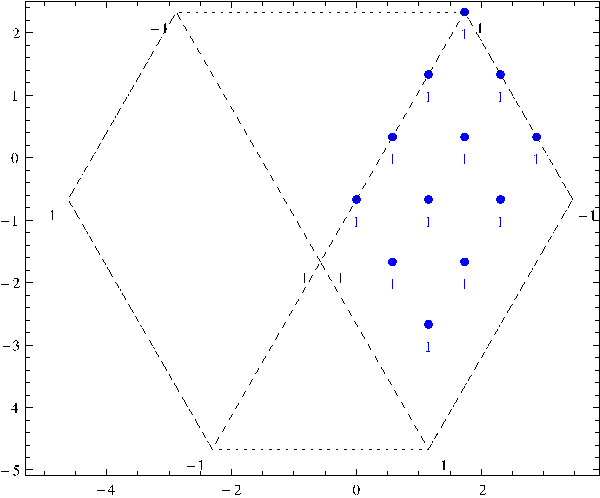
\includegraphics[width=80mm]{a2-a1}
  }
  \caption{Weyl group orbit (dotted) producing singular element of $L^{[3,2]}_{A_{2}}$ and its decomposition into the sum of splint images of singular elements of modules  $L^{[3,2]}_{A_{1}\oplus A_{1}}$ (dashed). Weight multiplicities of $L^{[3,2]}_{A_{1}\oplus A_{1}}$-module coincide with branching coefficients for the reduction $L^{[3,2]}_{A_{2}\downarrow A_{1}\oplus u(1)}$.}

 \label{fig:a2_splint}
\end{figure}
\end{example}



Consider Lie algebra $\gf$ and its irreducible modules $L^{\mu}_{\gf}$. 
Splints of root systems were introduced by D. Richter in paper \cite{richter2008splints} to describe cases of drastic simplification of module reduction into the sum of subalgebra modules. In paper \cite{2011arXiv1111.6787L} we've proved that branching coefficients coincide with multiplicities of the representation of second stem algebra.



In present note we generalize our analysis to affine extension of $\gf$. We consider affine Lie algebra $\gfh$ with the underlying simple finite-dimensional Lie algebra $\gf$. We assume that root system $\Delta_{\gf}$ admits splint $\Delta_{\gf}=\Delta_{\af_{1}}\cup \Delta_{\af_{2}}$. It is well-known \cite{kac1990idl} that irreducible $\gfh$-module can be decomposed into the sum of irreducible $\gf$-modules.
\begin{equation}
  \label{eq:1}
  L_{\gfh}^{\mu}=\bigoplus_{\nu=(\co{\nu},n,k)} b^{\mu}_{\co{\nu}}(n) L^{\co{\nu}}_{\gf}
\end{equation}

Then each of these $\gf$-modules in this decomposition admits decomposition to $\af_{1}$ modules with branching coefficients equal to weight multiplicities of $\af_{2}$ irreducible module \cite{2011arXiv1111.6787L}. 
\begin{equation}
  \label{eq:2}
  L^{\co{\nu}}_{\gf} = \bigoplus b^{\mu}_{\af_{1}\co{\nu}}(n) L^{\co{\nu}}_{\gf}
\end{equation}
We state that it is possible to reorganize weights in such a way that branching coefficients for the reduction $\gfh\downarrow \af_{1}$  are expressed in terms of weight multiplicities of $\hat\af_{2}$. 
\section{Main theorem}
\label{sec:main-theorem}

When an injection is maximal the
projection becomes trivial and the relation (\ref{recurrent rel}) is
simplified:
\begin{equation}
\begin{array}{c}
b_{\xi }^{\left( \mu \right) }=-\frac{1}{s\left( \gamma _{0}\right) }\left(
\sum_{u\in W}\epsilon (u) \delta _{\xi -\gamma _{0}, u(\mu +\rho )-\rho
}+\right. \\
\left. +\sum_{\gamma \in \Gamma _{\frak{a}\rightarrow \frak{g}}}s\left(
\gamma +\gamma _{0}\right) b_{\xi +\gamma }^{\left( \mu \right) }\right) .
\end{array}
\label{recurrent relation max}
\end{equation}
The recursion is goverened by the set $\Gamma _{\frak{a}\rightarrow \frak{g}}
$ called the injection fan. The latter is defined by the carrier set $%
\left\{ \xi \right\} _{\frak{a}\rightarrow \frak{g}}$ for the coefficient
function $s(\xi )$
\[
\left\{ \xi \right\} _{\frak{a}\rightarrow \frak{g}}:=\left\{ \xi \in P_{%
\frak{a}}|s(\xi )\neq 0\right\}
\]
appearing in the expansion
\begin{equation}
\prod_{\alpha \in \Delta ^{+}\setminus \Delta _{\frak{a}}^{+}}\left( 1-e^{
-\alpha }\right) =-\sum_{\gamma \in P_{\frak{a}}}s(\gamma )e^{-\gamma };\quad
\label{product}
\end{equation}

\begin{theorem}

 So following statement holds:
\begin{statement}
\label{statement-1}
\begin{equation}
\frac{e^{\rho _{\frak{g}}}}{\prod_{\beta \in \Delta _{\frak{s}%
}^{+}}(1-e^{-\beta })}\left( \Psi ^{\widetilde{\mu }+\rho _{\frak{s}%
}}\right) =\sum_{\widetilde{\nu }\in \mathcal{N}_{\frak{s}}^{\widetilde{\mu }%
}}M_{\left( \frak{s}\right) \widetilde{\nu }}^{\widetilde{\mu }}e^{\left(
\mu -\phi \left( \widetilde{\mu }-\widetilde{\nu }\right) \right)
}=\sum_{\nu \in P_{\frak{a}}^{++}}b_{\nu }^{(\mu )}e^{\nu }.
\label{singular main-4}
\end{equation}
Any weight with nonzero multiplicity in the r. h. s. is equal to one of the
highest weights in the decomposition. The multiplicity $M_{\left( \frak{s}%
\right) \widetilde{\nu }}^{\widetilde{\mu }}$ of the weight  $\widetilde{\nu
}\in \mathcal{N}_{\frak{s}}^{\widetilde{\mu }}$ defines the branching
coefficient $b_{\nu }^{(\mu )}$ for the highest weight $\nu =\left( \mu
-\phi \left( \widetilde{\mu }-\widetilde{\nu }\right) \right) $:
\[
b_{\left( \mu -\phi \left( \widetilde{\mu }-\widetilde{\nu }\right) \right)
}^{(\mu )}=M_{\left( \frak{s}\right) \widetilde{\nu }}^{\widetilde{\mu }}.
\]
\end{statement}


The extension to the case of non-twisted affine Lie algebras is not straightforward. The statement \ref{statement-1} is based upon the decomposition of the injection fan and the possibility to present the singular element of the algebra module as the linear combination of singular elements of second stem algebra modules. 

  Consider reduction of affine Lie algebra $\gfh$-module $L^{\mu}_{\gfh}$ to finite-dimensional subalgebra $\af_{1}$. Then for branching coefficients following relation holds:
  \begin{equation}
    \label{eq:3}
    b^{\mu}_{\nu}=\sum_{?} m^{\nu}_{\hat\af_{2}}
  \end{equation}
\end{theorem}
\begin{proof}
  At first we use equation \eqref{eq:1}, then substitute to equation \eqref{eq:2}, reorganize weights and obtain the desired result. 
\end{proof}

\section{Examples}
\label{sec:examples}
The most simple example is constructed starting with splint $\Delta_{A_{2}}=\Delta_{A_{1}\oplus A_{1}}\cup \Delta_{A_{1}}$.

Then we consider the case $\gfh=\hat B_{2}$.
\section*{Conclusion}
\label{sec:conclusion}
Further question is to generalize this analysis to affine sublagebras and apply the results on branching coefficients to the study of CFT coset models. 

%%  
%%  
%%  In the present paper we provide alternative proof of the main statement of paper [LN-2011-Splints] which uses graded commutative structure on vector space of universal enveloping algebra $U(n^{-})$. 
%%  
%%  Con
%%  
%%  
%%  Consider decomposition of simple Lie algebra $\gf=\nfp\oplus \hf \oplus \nfm$. Verma module $M^{\mu}=U(\gf)\underset{U(\bff_{+})}{\otimes} D^{\mu}(\bff_{+})$. $S(\nfm)=\{x_{1}\dots x_{l}:x_{i}\in\nfm\}_{l=0}^{\infty}$
%%  \begin{theorem}
%%    Fix some ordering $\alpha_{1},\dots,\alpha_{s}$ on the set of positive roots $\Delta^{+}$ and obtain the ordering on the basis $f_{1},\dots,f_{s}$ of $\nfm$.  Then monomials $f_{1}^{n_{1}} \dots f_{s}^{n_{s}}$ form a basis in $U(\nfm)\sim M^{\lambda}$ and $U(\nfm)\sim \mathbb{Z}^{s}_{\geq 0}$. 
%%  \end{theorem}
%%  \begin{statement}
%%    Let $\Delta^{+}_{\gf}=\Delta^{+}_{\af_{1}}\cup \Delta^{+}_{\af_{2}}$ be a splint positive root system of simple Lie algebra $\gf$. Then $M^{\lambda}_{\gf}\sim M^{\lambda}_{\af_{1}}\oplus M^{\lambda}_{\af_{2}}$.
%%    \begin{proof}
%%      Basis of $M^{\lambda}_{\gf}$ is given by $f_{1}^{n_{1}}\dots f_{s_{1}}^{n_{s_{1}}} f_{s_{1}+1}^{n_{s_{1}+1}}\dots f_{s_{1}+s_{2}}^{n_{s_{1}+s_{2}}}$, where $f_{1},\dots, f_{s_{1}}\in \nfm_{\af_{1}}$ and $f_{s_{1}+1},\dots,f_{s_{1}+s_{2}}\in \nfm_{\af_{2}}$
%%    \end{proof}
%%  \end{statement}
%%  Now consider irreducible $\gf$-module $L_{\gf}^{\mu}=M^{\mu}_{\gf}/I^{\mu}_{\gf}$t
%%  
\bibliography{bibliography}{}
\bibliographystyle{utphys}

\end{document}
